\section{内部原理}

\begin{frame}[fragile]{数据存储格式(一)}
    \begin{itemize}
        \item 数据存储的核心是一个\en{KV}数据库
        \item 数据单位通过\en{SHA1}散列值进行寻址
        \item 整体结构类似于\en{UNIX}文件系统布局
    \end{itemize}

    \begin{lstlisting}
    $ cd .git/objects && find . -type f

    ./1f/7a7a472abf3dd9643fd615f6da379c4acb3e3a
    ./83/baae61804e65cc73a7201a7252750c76066a30
    ./d6/70460b4b4aece5915caf5c68d12f560a9fe3e4
    \end{lstlisting}
\end{frame}

\begin{frame}{数据存储格式(二)}
    \centering
    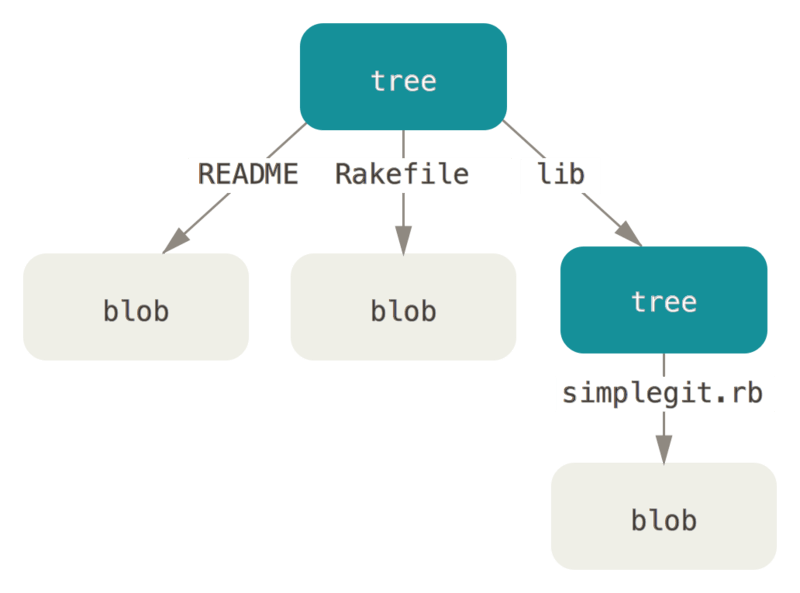
\includegraphics[scale=0.32]{figures/data-model-1.png}
\end{frame}

\begin{frame}{数据存储格式(三)}
    \centering
    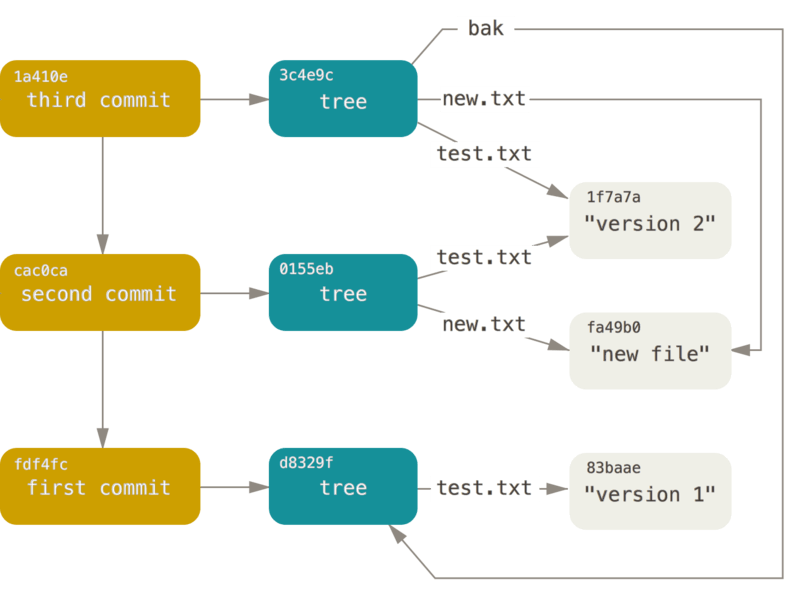
\includegraphics[scale=0.32]{figures/data-model-3.png}
\end{frame}

\begin{frame}{分支与标签的真相}
    \centering
    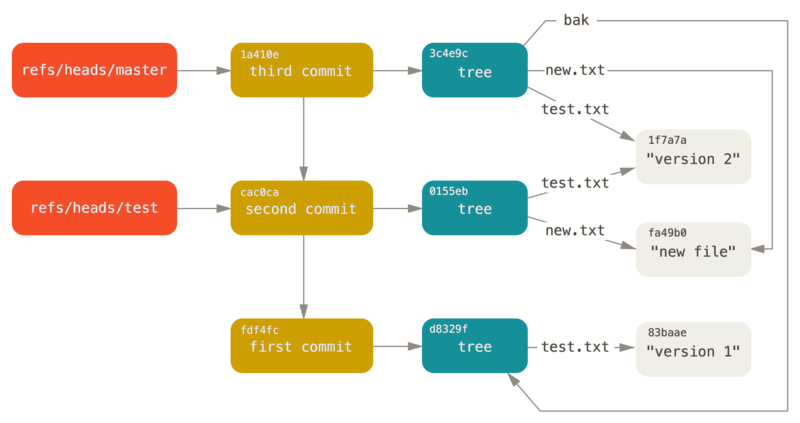
\includegraphics[scale=0.40]{figures/data-model-4.png}
\end{frame}
